\documentclass[a4paper]{article}

\usepackage[spanish]{babel}
\selectlanguage{spanish}

\usepackage[utf8]{inputenc}
\usepackage[T1]{fontenc}




\usepackage[a4paper,top=3cm,bottom=2cm,left=3cm,right=3cm,marginparwidth=1.75cm]{geometry}


\usepackage{amsmath, amsthm, amsfonts}

\usepackage{graphicx}
\usepackage[colorinlistoftodos]{todonotes}
\usepackage[colorlinks=true, allcolors=blue]{hyperref}

\usepackage[backend=biber]{biblatex}
\bibliography{referencias}

\title{Universidad 4.0}
\author{Armijo, Daniela\\
  \small daniarmijo@icloud.com
  \and
  Calvo, Nicolás\\
  \small ricardocalvo1997@gmail.com
  \and
  Kudaka, Matias\\
  \small matiaskudaka@gmail.com
  \and
  Olmedo, Matías\\
  \small olmedomn@live.com.ar
  \and
  Orozco, Marianela\\
  \small orozcomarianela10@gmail.com\\
  \small Universidad Tecnológica Nacional\\
  \small San Rafael - Mendoza
  \and
  Ramirez, Beatriz\\
  \small beatriz.vgb@gmail.com\\
  \date{}
}

\begin{document}

\begin{titlepage}
\centering
{\bfseries\LARGE Universidad Tecnológica Nacional \par}
\vspace{1cm}
{\scshape\Large Facultad Regional San Rafael\par}
\vspace{3cm}
{\itshape\Large Tecnicatura Universitaria en Programación \par}
\vspace{3cm}
{\scshape\Huge Hackaton: Universidad 4.0 \par}
\vfill
{\Large Grupo \par}
{\Large CODEPEOPLE \par}
\vfill
{\Large Diciembre 2022 \par}
\end{titlepage}

\tableofcontents

\maketitle

\begin{abstract}
Los problemas que se encuentran durante el proceso de inscripción y cursado en la FRSR, pueden resolverse aprovechando los avances tecnológicos.
\end{abstract}

\twocolumn

\section{Planteamiento del problema}

Hoy en día la administración pública permite acceder a una gran variedad de trámites en línea, como gestionar la renovación del DNI, el certificado de antecedentes personales y mucho más, simplemente haciendo uso de distintas aplicaciones. Todo esto se puede hacer desde un dispositivo móvil o computadora, para lo que se necesita de los sistemas informáticos, las aplicaciones móviles, las redes informáticas y muy especialmente la seguridad. Pero aún hoy en día, un número importante de gestiones se deben hacer en forma personal. Y en un sinnúmero de estas se solicitan certificados o formularios que debemos imprimir o fotocopiar, o más aún, retirarlos de alguna oficina o registro, con el pago de algún sellado. Por ejemplo, para realizar algunas se solicita la partida nacimiento, legalizada con una antigüedad no mayor a 3 meses. Esto obliga a ir al Registro correspondiente, hacer cola, solicitarla, pagar un código en otro lugar y volver a retirarla. Burocracia, papeleo, firmas en papel, esto no sería necesario si contásemos con un sistema único donde estén todos nuestros datos almacenados, de donde podamos obtenerlos y transmitirlos de una institución a otra sin necesidad de oficinas intermediarias minimizando el gasto de recursos. El uso de diferentes sistemas tampoco es lo óptimo. 

Llevando esto al plano de la facultad regional San Rafael de la UTN, donde se realiza el estudio, se observa que sucede algo similar. Los problemas con la Tecnicatura Universitaria en Programación se han generado porque falta un sistema que controle el volumen de información que generan/solicitan más de 500 personas. Teniendo en cuenta que en el período 2011-2022 la cantidad de estudiantes que eligen carreras en modalidad virtual creció un 64,5\% y la cantidad de egresados de esta modalidad un 190,3 \%, ~\cite{blearning} estos problemas van a ir en aumento. Se enumeran algunos de ellos.

El proceso de inscripción es lento, se solicitan fotocopias de DNI, títulos, rellenar formularios y llevarlos en persona a la institución. Ya existe un sistema (miArgentina) que tiene los datos personales, DNI digital, etc. que se utilizan en este proceso. De la misma manera, la Dirección General de Escuelas tiene un sistema (GEM) en el cual está toda la trayectoria escolar de los estudiantes.  El sistema de inscripción a la facultad debería recurrir a estos para tomar los datos de los aspirantes, sin necesidad de recurrir al papel, viajes hasta el lugar, lugar físico para guardar legajos, personas para gestionar el proceso, etc. Son gastos que podrían reducirse o eliminarse. Incluso contar con un sistema de toma de medidas biométricas, para reconocimiento facial, y de toma de firmas electrónicas legales. El lugar físico debería reemplazarse por “nubes” para guardar los datos que son “espacios virtuales” que, aunque también generan gastos, son menores, considerando también el mantenimiento y luego el peligro y riesgos que implica mantener en una institución volúmenes importantes de legajos en papel. Ha pasado que en instituciones se han perdido por incendios e inundaciones. Obviamente que el resguardo de datos en la nube también implica el uso de seguridad informática, pero es menos propenso a riesgos y a pérdidas, filtrado, etc. 

El problema que acarrea estos trámites continúa al momento de rendir un examen final. Las inscripciones se realizan por sistema, pero el sistema es susceptible de errores. Los estudiantes se quejan del mismo, no es claro, se inscriben y no aparecen, etc. Luego los profesores no tienen un sistema para asentar las notas, las notas se pasan por escrito en una planilla, por cada especialidad va una planilla por duplicado, la misma luego tienen que firmarla los docentes y luego se vuelca al sistema. Esto genera atrasos, errores y hasta pérdidas de información. Además de que se presta a manejos indeseables.  

El sistema académico que así se llama, aunque tiene la capacidad para registrar varios datos, no se usa en su totalidad. Los docentes deben llevar cada uno un listado de sus alumnos, con la información que los alumnos estén dispuestos a brindar, para tomar asistencia, colocar notas y observaciones. Lo ideal sería contar son un sistema que permita a cada profesor acceder a la trayectoria de cada alumno, colocar sus asistencias y notas. Un sistema que sea igual para todas las cátedras, automático, calculando porcentajes de asistencia, promedios, y que le asigne automáticamente a cada alumno su estado (libre, regular, aprobado).
Esto implicaría un ahorro significativo en: espacio físico, personal, artículos de librería y oficina, etc. Simultáneamente la eficiencia del sistema sería mayor. 

La problemática se presenta también en la extensión de título. Por sistema, el ya graduado no tendría que esperar tiempo para recibir su título. Automáticamente, rinde su última materia y se asienta en sistema, el título digital está a su disposición, con la misma validez que el físico, el cual ya no sería necesario, ahorrando de esta manera además de tiempo, dinero. Esto exige, como en cada etapa de este sistema, la completa seguridad del mismo. 


\section{La propuesta. Misión}

Se propone el desarrollo de un sistema de acuerdo con estándares internacionales de seguridad que garantice el cumplimiento de los requisitos de seguridad y calidad para realizar todas las tareas administrativas, entre otras, que deben hacer los actores de  la institución. En el mismo, los datos personales se almacenarán y manejarán con confidencialidad e integridad.  

\subsection{Objetivos}

Los objetivos de la propuesta son:
\begin{enumerate}
\item Reducir el número de empleados que realizan estas tareas manualmente
\item Desarrollar procesos (contables, de inscripciones, de certificaciones, etc) sin papel, eficaces y automatizados.
\item Lograr que los datos de gestión, personales, etc. estén centralizados y disponibles a nivel de cualquier institución que los necesite, actualizados y en tiempo real, con un nivel de seguridad máximo.
\end{enumerate}

\subsection{Visión} 

Consolidar un sistema a nivel nacional amplio y articulado, de fácil acceso, con un flujo de información mas óptimo y eficiente. Evitar presentación de papeles, fotocopias, rellenado de formularios, sellados, pagos, duplicación de información, etc. 

Un ejemplo a nivel mundial ha sido desarrollado con éxito en Estonia; lo llaman proyecto de centralización de los servicios compartidos estatales. “En el punto de partida había 253 agencias estatales con contabilidad financiera independiente, contabilidad de recursos humanos y sistemas de cálculo de nómina. Había 14 soluciones de software de contabilidad diferentes y 11 soluciones de software de contabilidad de recursos humanos diferentes en uso y no había un sistema de informes común. Los sistemas informáticos de función principal no estaban vinculados a software de contabilidad financiera o de personal. Todas las agencias gastaron dinero por separado en el desarrollo de esos diferentes softwares.” ~\cite{estonia}
Como resultado de la aplicación del proyecto de sistematización y unificación de los sistemas informático, se ha reducido el número de empleados, se ha centralizado la información, los empleados estatales están satisfechos porque se ha reducido la burocracia por lo que los procesos son mucho más rápidos. También se ha logrado una importante reducción de la corrupción en el estado. Para visualizar la diferencia entre ambos países, usamos el Indice de Percepción de la Corrupción, publicados por Transparecy Internacional, como puede verse en la fig. \ref{fig:Imagen1}.

\begin{figure}
\centering
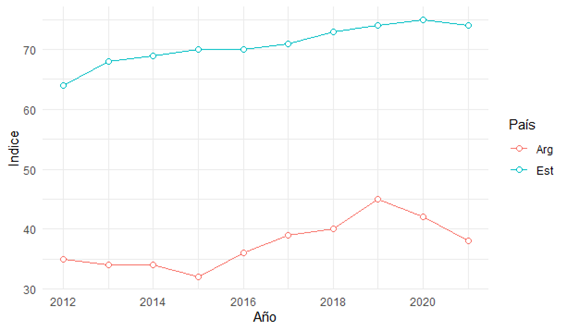
\includegraphics[width=0.5\textwidth]{Imagen1.png}
\caption{\label{fig:Imagen1}Indice de Percepción de la Corrupción.}
\end{figure}

“El Índice de Percepción de la Corrupción clasifica 180 países y territorios según el nivel de percepción de la corrupción en el sector público de cada uno, en una escala de cero (muy corruptos) a cien (muy limpios).” ~\cite{ipc}

Para la implementación de un centro de similares características, son necesarios algunos pasos previos, como educación del ciudadano en sistemas, conectividad en el país, desarrollo de software apropiado asociando el sistema público con empresas privadas, unificando sistemas. 

\section{Estudio de mercado}

La pregunta que surge es: ¿Está preparado el mercado para este cambio? Para responder a esta pregunta, se realiza un relevamiento de información mediante tres herramientas: 

\begin{enumerate}
\item Una encuesta online realizada a través de formularios de Google
\item Entrevistas desestructuradas realizadas a miembros de la comunidad educativa (docentes, administrativos, alumnos)
\item Observación
\end{enumerate}

\subsection{Resultados}

\begin{figure}
\centering
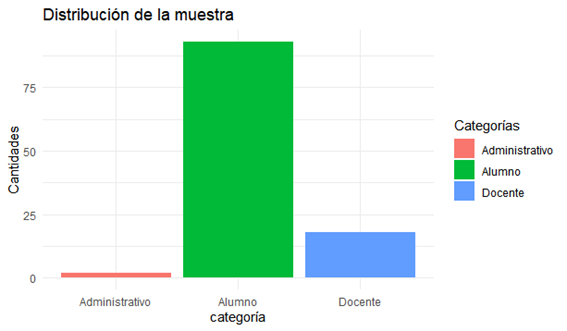
\includegraphics[width=0.5\textwidth]{Imagen2.png}
\caption{\label{fig:Imagen2}Distribución de la muestra.}
\end{figure}

La encuesta fue respondida por 113 personas, entre alumnos, docentes y administrativos. El análisis de los datos se realiza usando R. En la fig. \ref{fig:Imagen2} puede observarse la distribución de la muestra.

La muestra tiene una mayoría de alumnos. Es posible que los resultados obtenidos tengan un “sesgo” por el rango etario de los alumnos.

A continuación, la encuesta preguntaba sobre el uso que hacen tanto docentes como alumnos y administrativos de los servicios en línea, utilizando una escala lineal, donde 1 implica que nunca hacen trámites en línea y 5, que siempre lo hacen. Los resultados, independientemente de la categoría, pueden verse en la fig. \ref{fig:Imagen3}

\begin{figure}
\centering
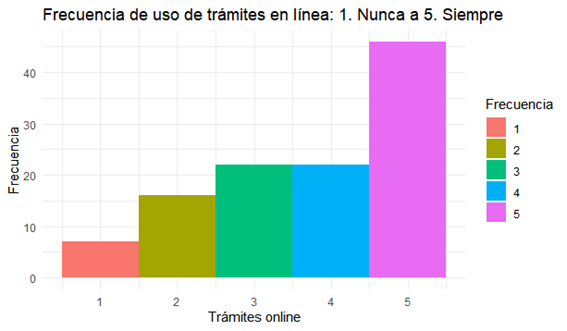
\includegraphics[width=0.5\textwidth]{Imagen3.png}
\caption{\label{fig:Imagen3}Uso de servicios en línea.}
\end{figure}

Como puede observarse, el histograma permite ver una distribución sesgada a la izquierda, con la mayoría de los valores agrupados en la opción 5, es decir, quienes realizan todos los trámites que pueden en línea. 

Sin embargo, hay un número de personas que aún no realizan todos los trámites en línea. Es por eso que, una de las cuestiones involucradas en la propuesta es la educación digital del ciudadano para el uso de estas tecnologías. 

En ese sentido, se relevó la capacitación de los ciudadanos para el uso de estas tecnologías según el rango de edad (ver fig \ref{fig:Imagen4}). En el gráfico de barras puede observarse que, a medida que aumenta la edad, menor capacitación tienen los individuos. Esto tenderá a desaparecer naturalmente con el tiempo, cuando las generaciones sean todas nativos digitales, o se hayan adaptado a la digitalización.

\begin{figure}
\centering
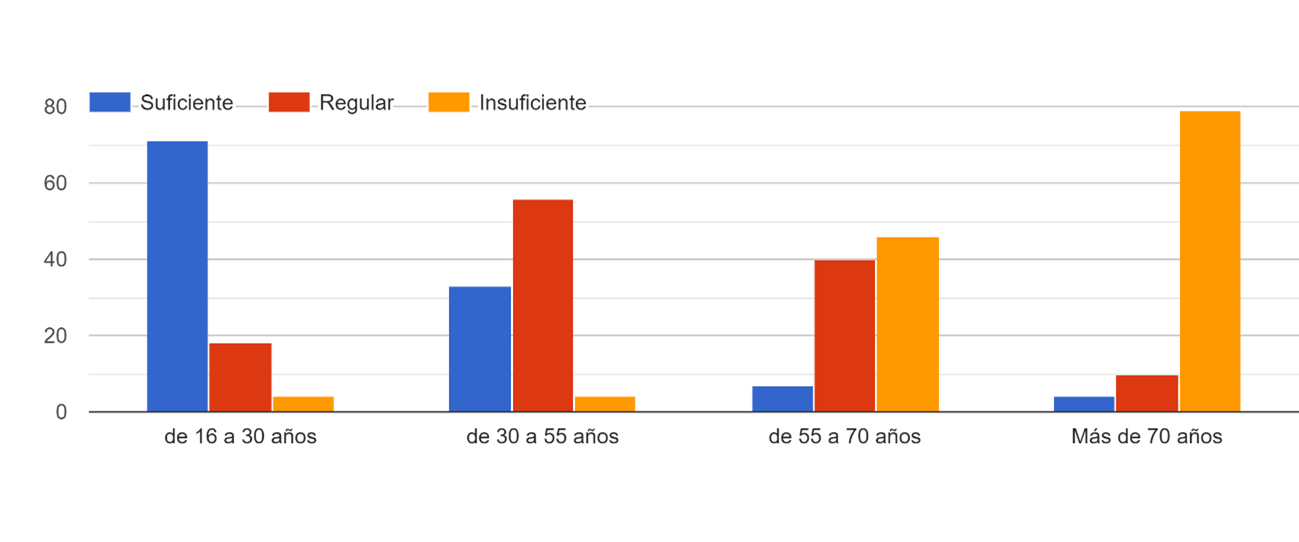
\includegraphics[width=0.5\textwidth]{Imagen4.png}
\caption{\label{fig:Imagen4}Capacitación digital de los ciudadanos según rango etario.}
\end{figure}

\subsubsection{Otros resultados}
\begin{figure}
\centering
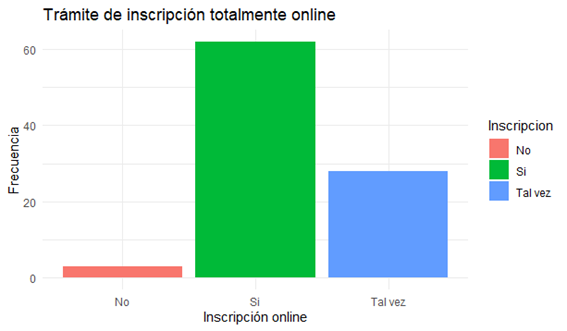
\includegraphics[width=0.5\textwidth]{Imagen5.png}
\caption{\label{fig:Imagen5}Trámite de inscripción en línea}
\end{figure}

Con respecto a los trámites a realizarse en la facultad, se plantean las siguientes preguntas:

¿El trámite de inscripción debería ser totalmente en línea? ver fig \ref{fig:Imagen5}. 

Las entrevistas informales nos permiten deducir que, los alumnos que superan el rango de los 35 años prefieren el formato presencial. Algunos estudiantes de menos de 20 años, aunque eligen el formato en línea, plantean también la necesidad de una atención presencial para recibir asesoramiento en persona. 

\begin{figure}
\centering
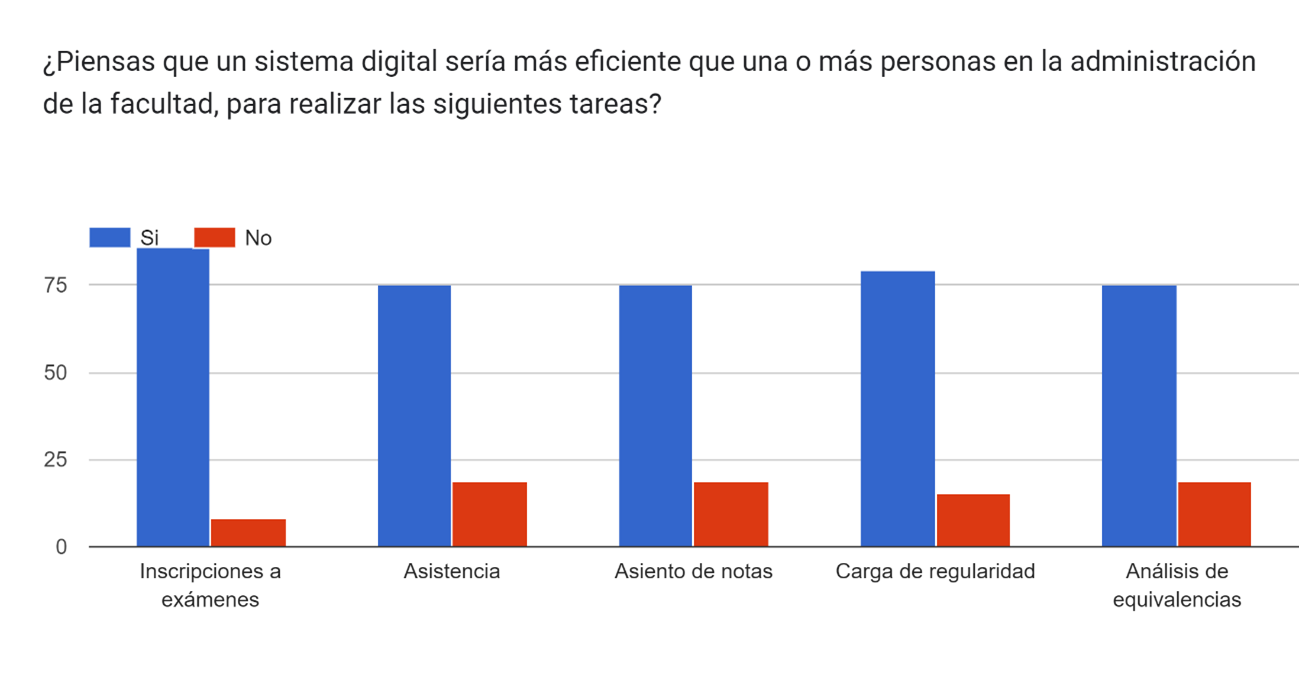
\includegraphics[width=0.5\textwidth]{Imagen6.png}
\caption{\label{fig:Imagen6}Eficiencia del sistema con otros trámites}
\end{figure}

Algunas de las tareas que realiza la parte administrativa fueron incluidas en la encuesta para que los alumnos respondieran si les parece que las mismas serían más eficientes realizadas por sistema. Las respuestas pueden verse en la fig \ref{fig:Imagen6}. También se preguntó acerca de la posibilidad de tener el título en formato digital (fig \ref{fig:Imagen7}). 

\begin{figure}
\centering
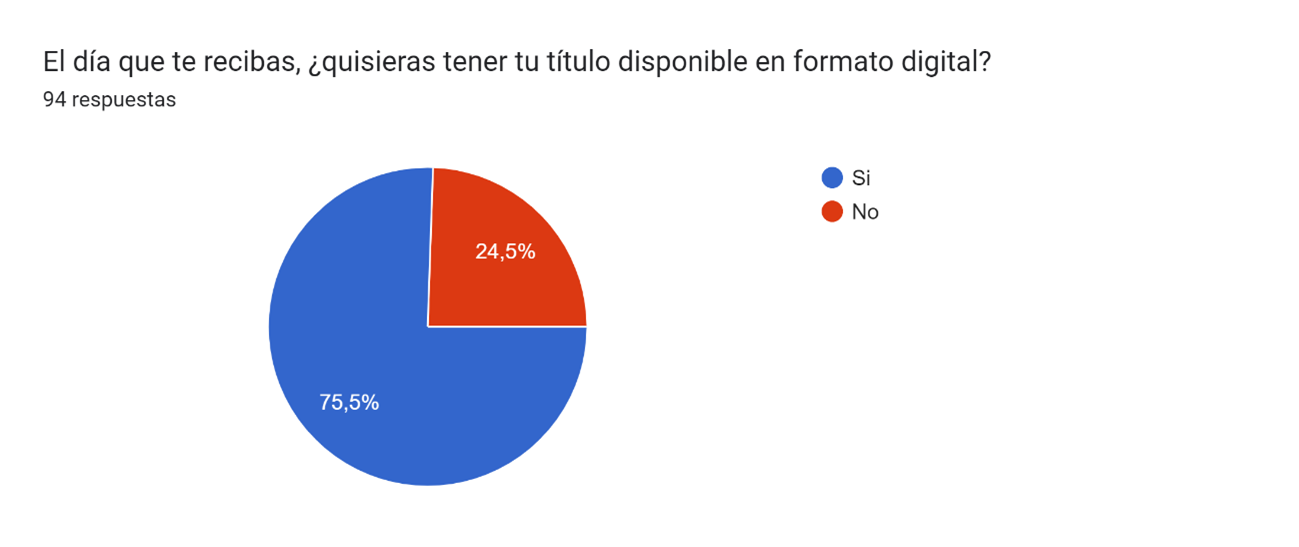
\includegraphics[width=0.5\textwidth]{Imagen7.png}
\caption{\label{fig:Imagen7}Títulos: ¿digitales o físicos?}
\end{figure}

En Mendoza, la Dirección General de Escuelas, ha adoptado un sistema donde se lleva el registro de la trayectoria académica de los alumnos. La fig \ref{fig:Imagen8} muestra que, quienes lo conocen, casi la mitad lo encuentra ineficiente. El sistema es relativamente nuevo, y ha ido mejorando año a año. Los docentes son, en general, quienes más se resisten, pero estimamos que esto es por la falta de capacitación en el uso de sistemas informáticos. 

\begin{figure}
\centering
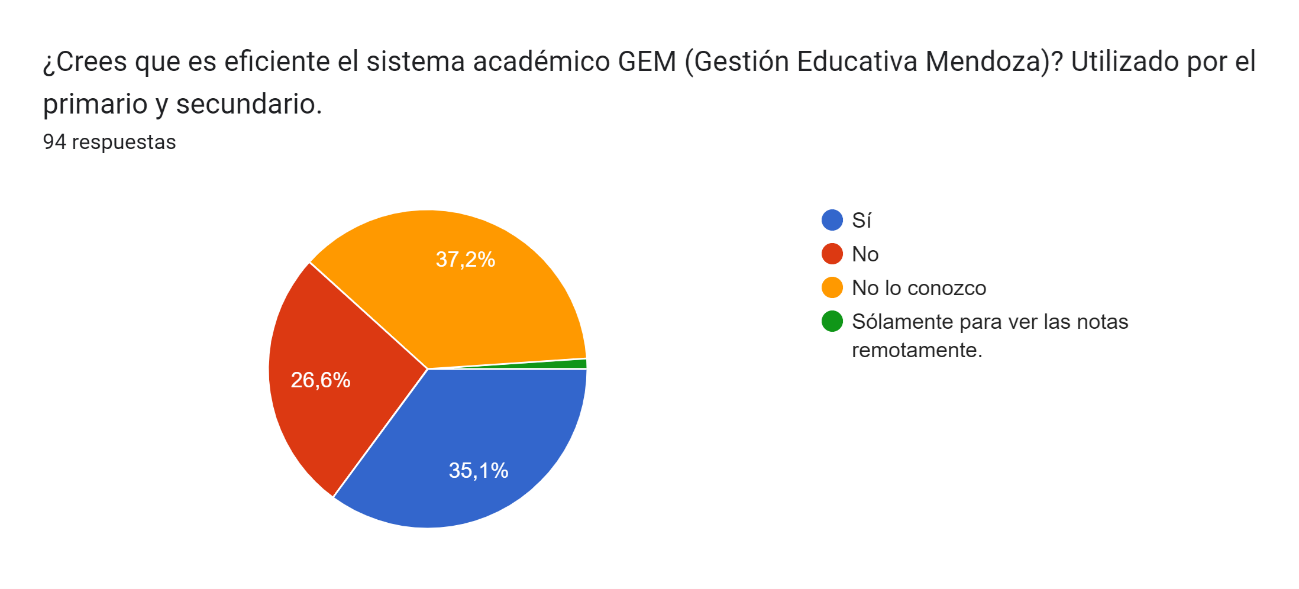
\includegraphics[width=0.5\textwidth]{Imagen8.png}
\caption{\label{fig:Imagen8}Eficiencia del sistema GEM.}
\end{figure}

Se sabe que implementar un sistema lleva su tiempo de mejoras, aprendizajes, y necesita una red de conectividad que es posible que no contemos aún en nuestro país. Razón más para insistir en la inclusión de estas tecnologías para obligar a la modernización del sistema y a la capacitación de los usuarios. No se puede pensar en crecer como instituciones, como empresas, como regiones, si no contamos con estas herramientas. 


\begin{figure}
\centering
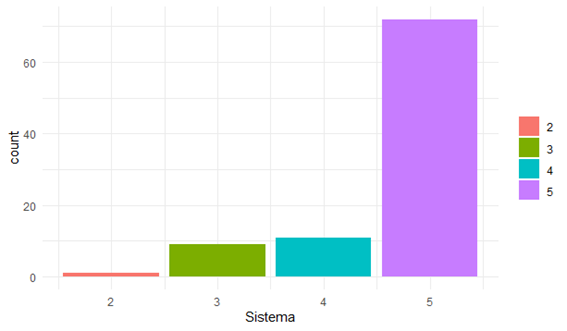
\includegraphics[width=0.5\textwidth]{Imagen9.png}
\caption{\label{fig:Imagen9}Solicitar y recibir documentación en línea.}
\end{figure}


Cuando se les pregunta a los alumnos qué tan útil le resultaría poder obtener toda la documentación necesaria (certificados, registros, actas, etc.) por sistema, en una escala lineal, de 1 a 5, donde 1 representa “nada útil” y 5 “muy útil”, observamos la distribución de frecuencias de la fig \ref{fig:Imagen9}.

\section{Análisis competitivo}

FODA son las siglas que representan al estudio de las Fortalezas, las Oportunidades, las Debilidades y las Amenazas de una empresa en un mercado. 
Realizamos la matriz FODA (ver fig \ref{fig:Imagen10}) de nuestra propuesta teniendo en cuenta que el objetivo es automatizar procesos convirtiéndolos en más eficientes y sustentables, logrando disminuir el uso de recursos económicos, humanos y de tiempo.

\begin{figure}
\centering
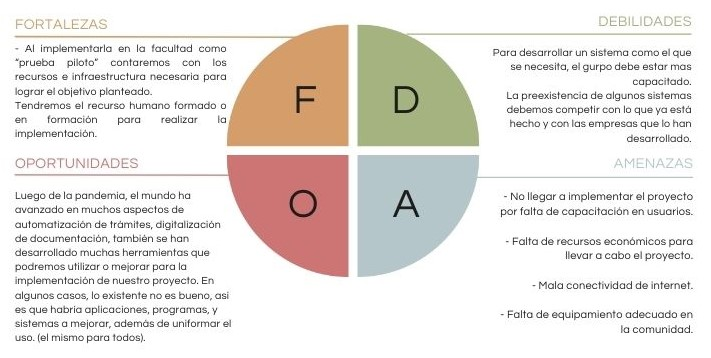
\includegraphics[width=0.5\textwidth]{Imagen10.jpg}
\caption{\label{fig:Imagen10}Matriz FODA.}
\end{figure}

\section{Conclusiones}

El análisis de estos datos y otros relevados, tanto en encuestas como en entrevistas informales, y la propia observación, muestran una tendencia al aumento en el uso de aplicaciones para realizar trámites, sin embargo, las personas aún muestran una confianza en la atención presencial, en la documentación escrita, y también muestran desconfianza en los sistemas informáticos. El desconocimiento o desinformación que se percibe aumenta esta sensación de inseguridad, sobre la que se debería trabajar para poder implementar exitosamente un sistema, tanto en la facultad como en otras instituciones y luego un sistema interconectado para todas las instituciones estatales y/o privadas. Es necesario que, como menciona ONU en el art. 9 de la Res. 70/125 (2015) los ciudadanos comprendan que “los mismos derechos de los que las personas gozan fuera de línea también deben ser protegidos en línea” ~\cite{onu15}. Que los datos personales y confidenciales estén en línea, no implicará en ningún momento que estén en peligro, si no más bien se asegurará que se amparen los derechos humanos y las libertades fundamentales. 
El Art. 9 de la Res. 70/1 2015 de la ONU expone “La expansión de las tecnologías de la información y las comunicaciones y la interconexión mundial brinda grandes posibilidades para acelerar el progreso humano, superar la brecha digital y desarrollar las sociedades del conocimiento…”~\cite{onu15}. Estamos convencidos que nuestro proyecto va en esa línea. 
También la ONU, en el art. 5 de la Res. 70/125  de 2015 segura que “la mayor conectividad, innovación y acceso a las tecnologías de la información y las comunicaciones ha desempeñado una función esencial a los efectos de facilitar los progresos en relación con los Objetivos de Desarrollo del Milenio …” ~\cite{onu15} mostrando así la importancia fundamental de contar con conectividad en todos los rincones del país. 

\onecolumn

\printbibliography

\end{document}